\documentclass[a4paper,10pt,twoside]{article}
\usepackage[utf8]{inputenc}
\usepackage[french]{babel}
\usepackage[T1]{fontenc}
\usepackage{amsmath}
\usepackage{amsfonts}
\usepackage{amssymb}
\usepackage{graphicx}
\usepackage{multicol}
\usepackage{array}
\usepackage{float}
\usepackage{epstopdf}
\usepackage[justification=centering]{caption}
\usepackage{caption}
\usepackage{subfig}
\usepackage{gensymb}
\usepackage[bottom]{footmisc}
\usepackage{appendix}
\usepackage{pdfpages}
\usepackage{todonotes}
\usepackage{mathpazo}
\usepackage{titleps}
\usepackage{color}
\usepackage{hyperref}
\usepackage[skins]{tcolorbox}
\usepackage{sectsty} 
\usepackage[arrowmos]{circuitikz}
\usepackage{pgfplots}
\usepackage{blindtext}
\usepackage{adjustbox}
\usepackage[inner=2.5cm,outer=2.5cm,top=3cm,bottom=3cm]{geometry}

\graphicspath{{pictures/}}
\setlength\parindent{0pt}
\renewcommand*\rmdefault{ppl}
\newcolumntype{C}[1]{>{\centering\let\newline\\\arraybackslash\hspace{0pt}}m{#1}}
\newcolumntype{R}[1]{>{\raggedright\arraybackslash}p{#1}}
\sectionfont{\large}
\subsectionfont{\normalsize}

% Page style definitions
\newpagestyle{main}{
	\sethead[Club ELEC : Quête de la balise RF][][]  % even
			{\chaptertitle}{}{Club ELEC : Quête de la balise RF}
	\headrule
    \setfoot[\thepage][][]
    		{}{}{\thepage}		
}

\newpagestyle{appendix}{
	\sethead[Club ELEC : Annexes][][]  % even
			{}{}{Club ELEC : Annexes}
	\headrule
    \setfoot[\thepage][][]
    		{}{}{\thepage}
    \footrule
}

%----------------------------------------------------------------------------------------
%	TITLE SECTION
%----------------------------------------------------------------------------------------
\title{	
	\vspace{2.5cm}
	\normalfont \normalsize 
	\huge Club ELEC\\ 
	\huge Quête de la balise RF de LLN\\
	\huge Phase 1 - Assemblage
	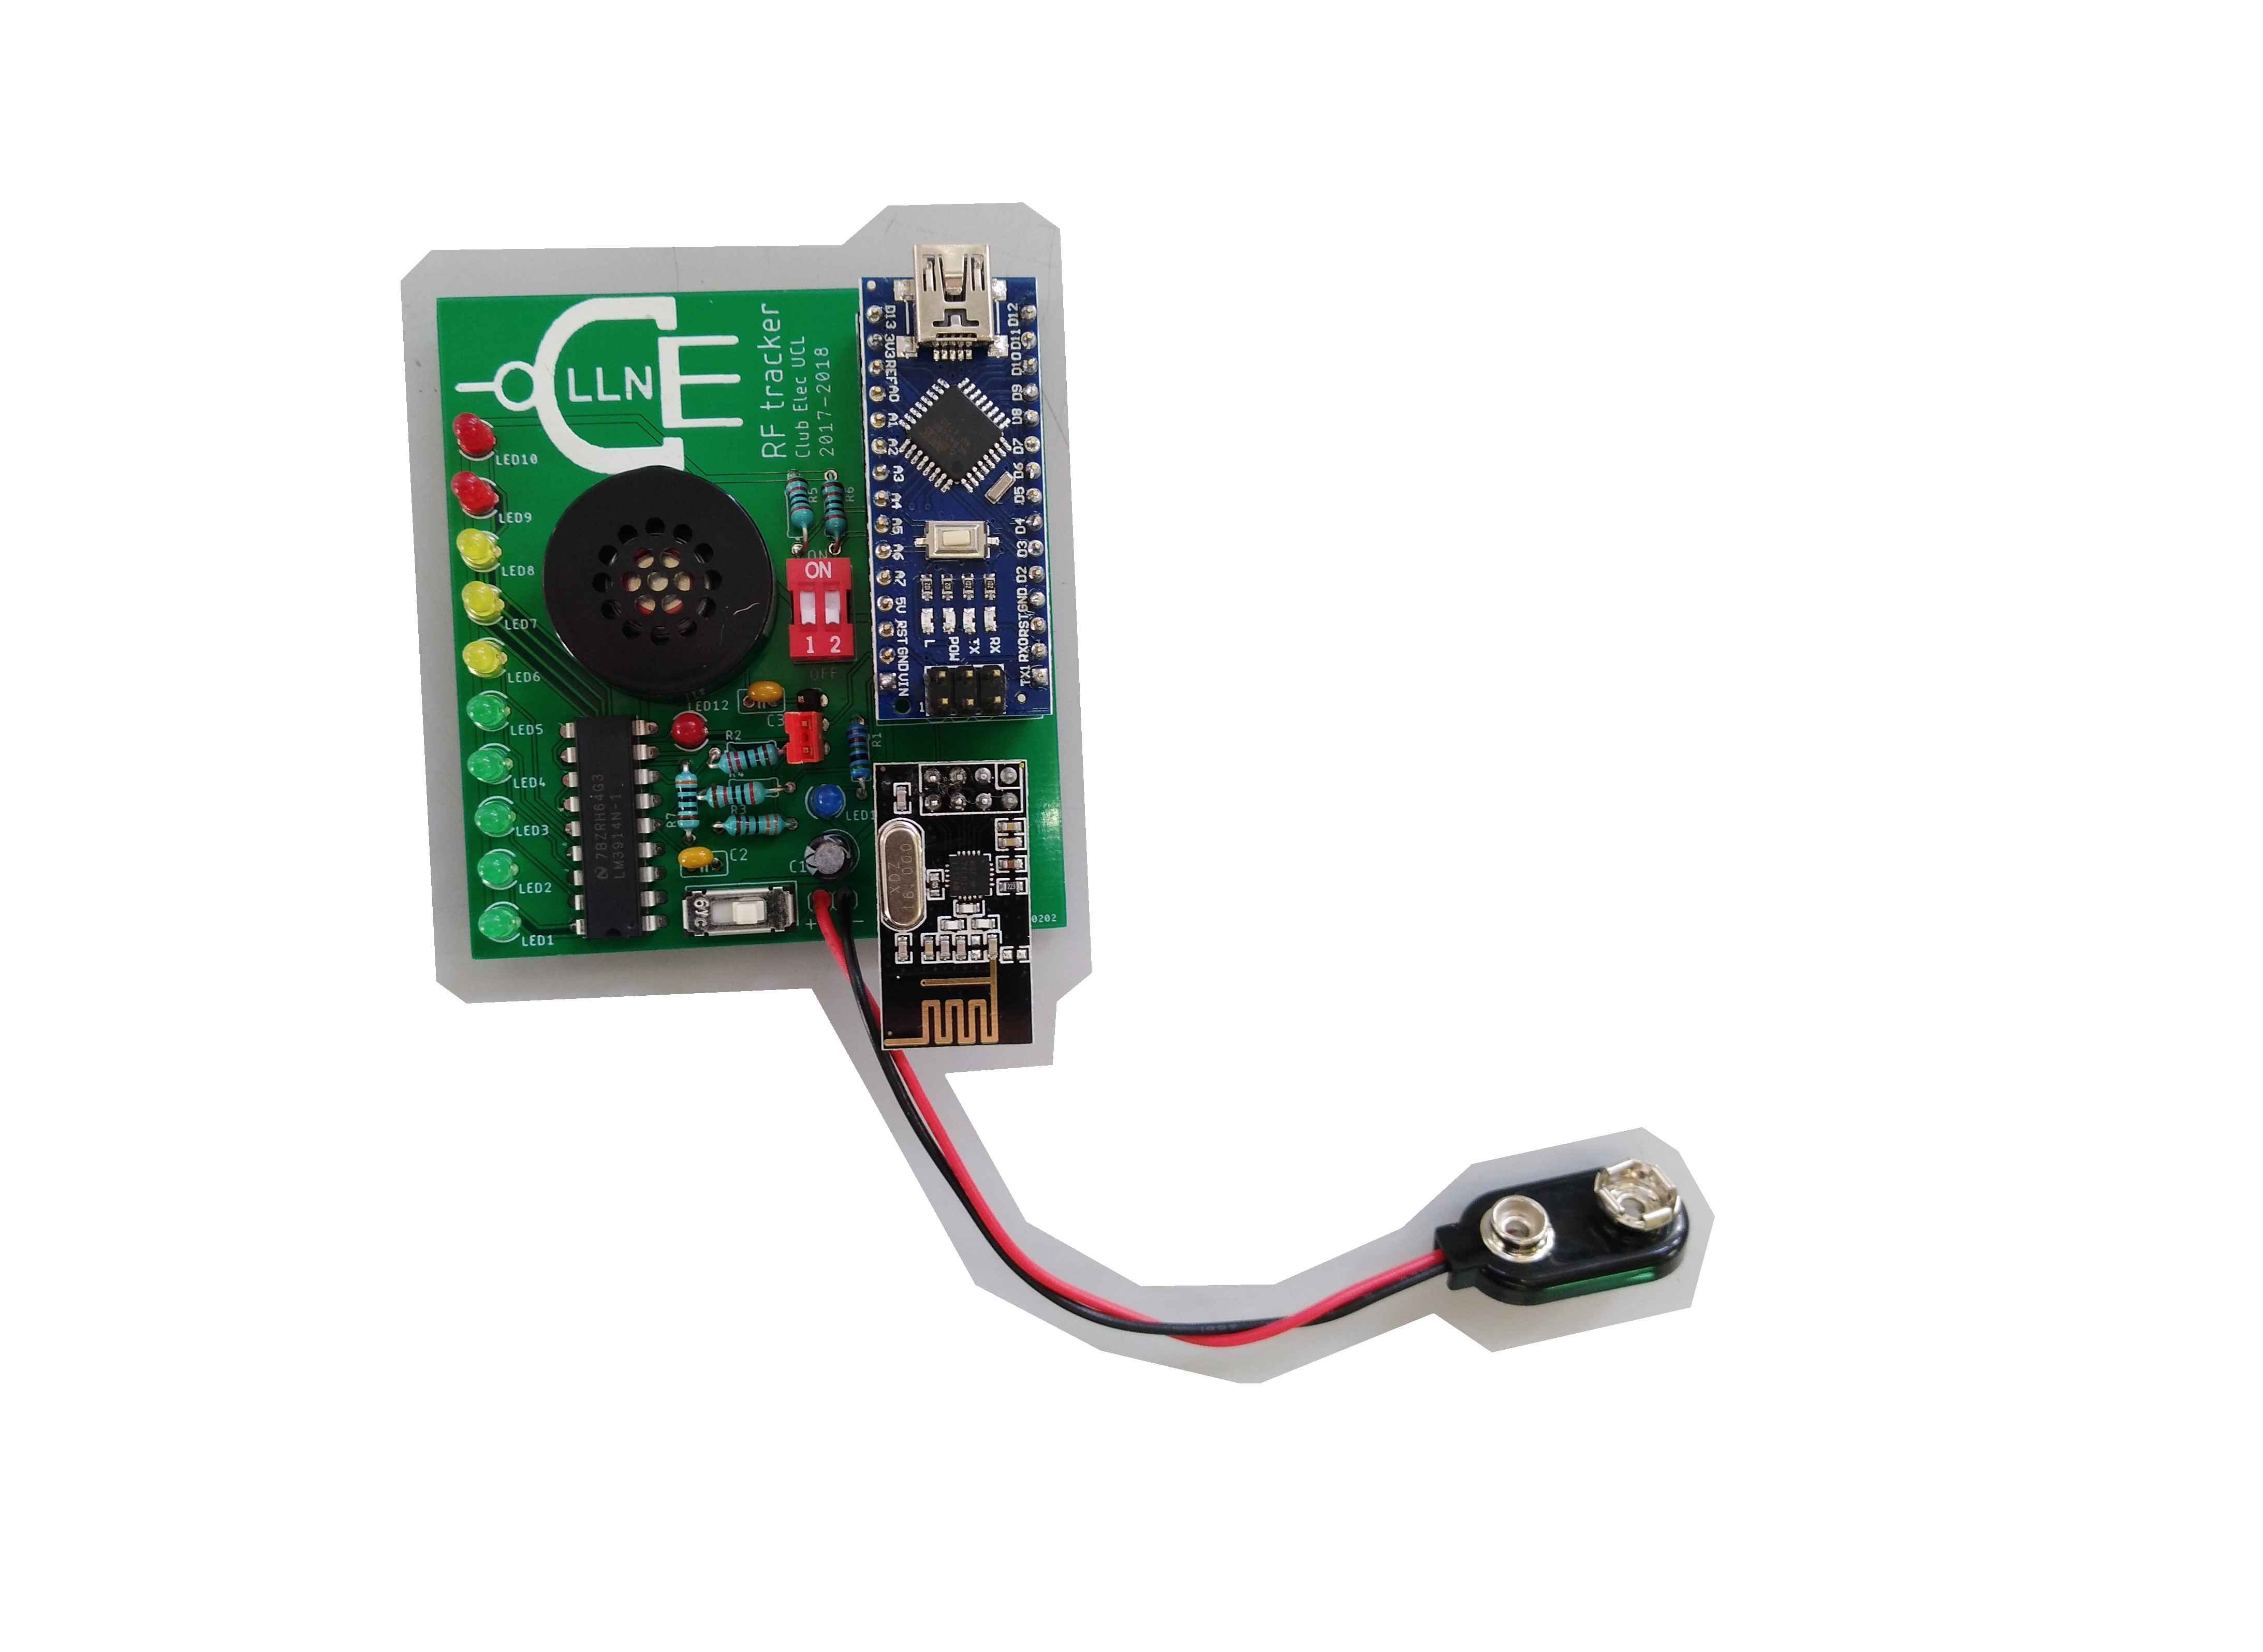
\includegraphics[width=.9\textwidth]{imgs/RF_TAG_withoutBackground.jpg}
	\vspace{2.5cm}
	\centering
}

\begin{document}
\renewcommand{\figurename}{Fig.}
\renewcommand{\thepage}{\roman{page}}
\setcounter{page}{1}

\pagenumbering{gobble}
\maketitle
\newpage
\pagenumbering{arabic}
\pagestyle{main}

\newpage
\null
\thispagestyle{empty}
\newpage
\clearpage

\setcounter{page}{1}

%%% Introduction
\section*{La Quête de la balise RF perdue dans Louvain-la-Neuve}

Bienvenue au Club ELEC pour le projet de ce quadrimestre, à savoir la \textit{Quête de la balise RF de Louvain-la-Neuve}! Nous avons besoin de vous! En effet, une \textbf{balise RF émettrice} a été perdue dans la ville de Louvain-la-Neuve. Votre mission, si vous l'acceptez? La localiser.\\ 

Pour accomplir cette mission, vous aurez tout d'abord besoin d'une ... \textbf{balise RF réceptrice}. À l'aide de celle-ci, vous pourrez correctement réceptionner les messages transmis par la balise perdue et la retrouver les premiers!
\\

Concrètement, le projet à réaliser sera subdivisé en 3 phases:\\
\begin{itemize}
	\item[$\bullet$] Phase 1: compréhension et assemblage de la balise RF réceptrice;
	\item[$\bullet$] Phase 2: programmation de la balise RF réceptrice;
	\item[$\bullet$] Phase 3: localisation de la balise RF perdue. \newline
\end{itemize}

Aujourd'hui, nous attaquons la \textbf{phase 1} de cette quête. L'objectif est d'assembler la balise RF réceptrice. En particulier, il s'agira de comprendre le fonctionnement du circuit et de souder les différents composants électroniques qui le constituent. A titre d'information, votre point de départ sera la Fig. \ref{fig:RF_TAG_components}, et ce à quoi vous devrez arriver est le résultat montré à la Fig. \ref{fig:RF_TAG}.\\

\begin{minipage}[c]{.49\textwidth}
	\centering
	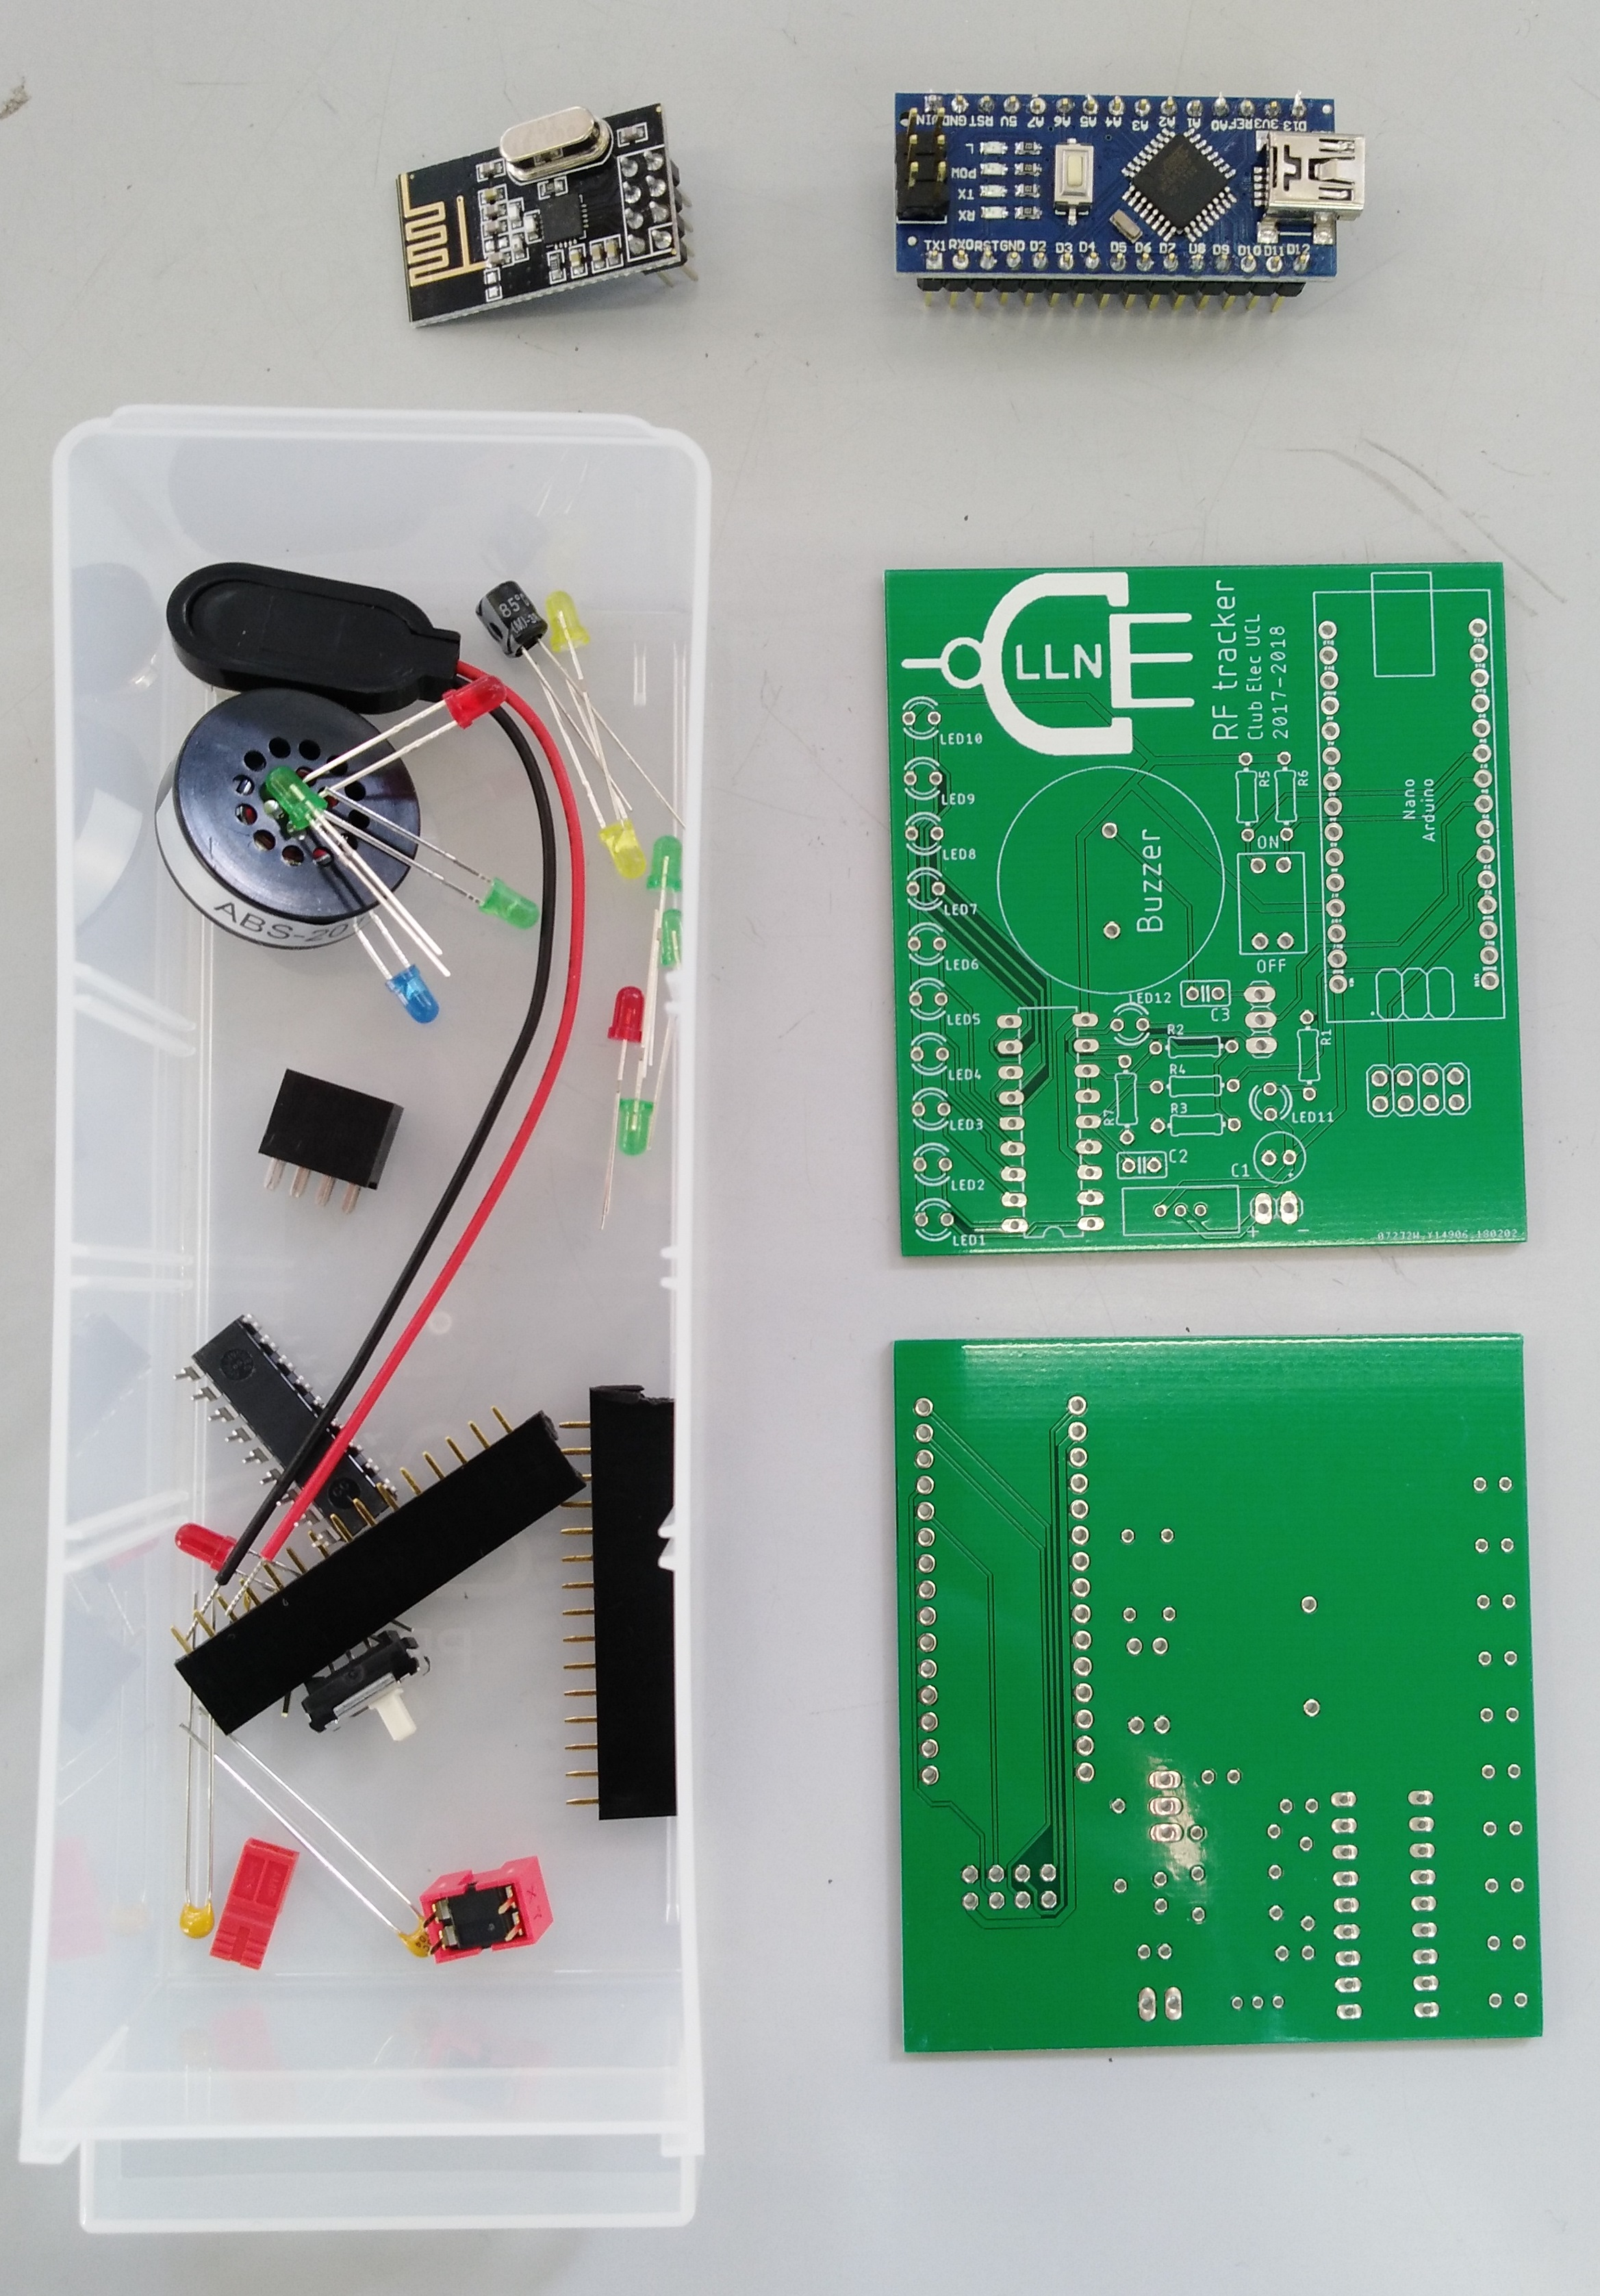
\includegraphics[width=\textwidth]{imgs/RF_TAG_components.jpg}
	\captionof{figure}{Point de départ : composants et circuit imprimé.}
	\label{fig:RF_TAG_components}
\end{minipage}
\hfill
\begin{minipage}[c]{.49\textwidth}
	\centering
	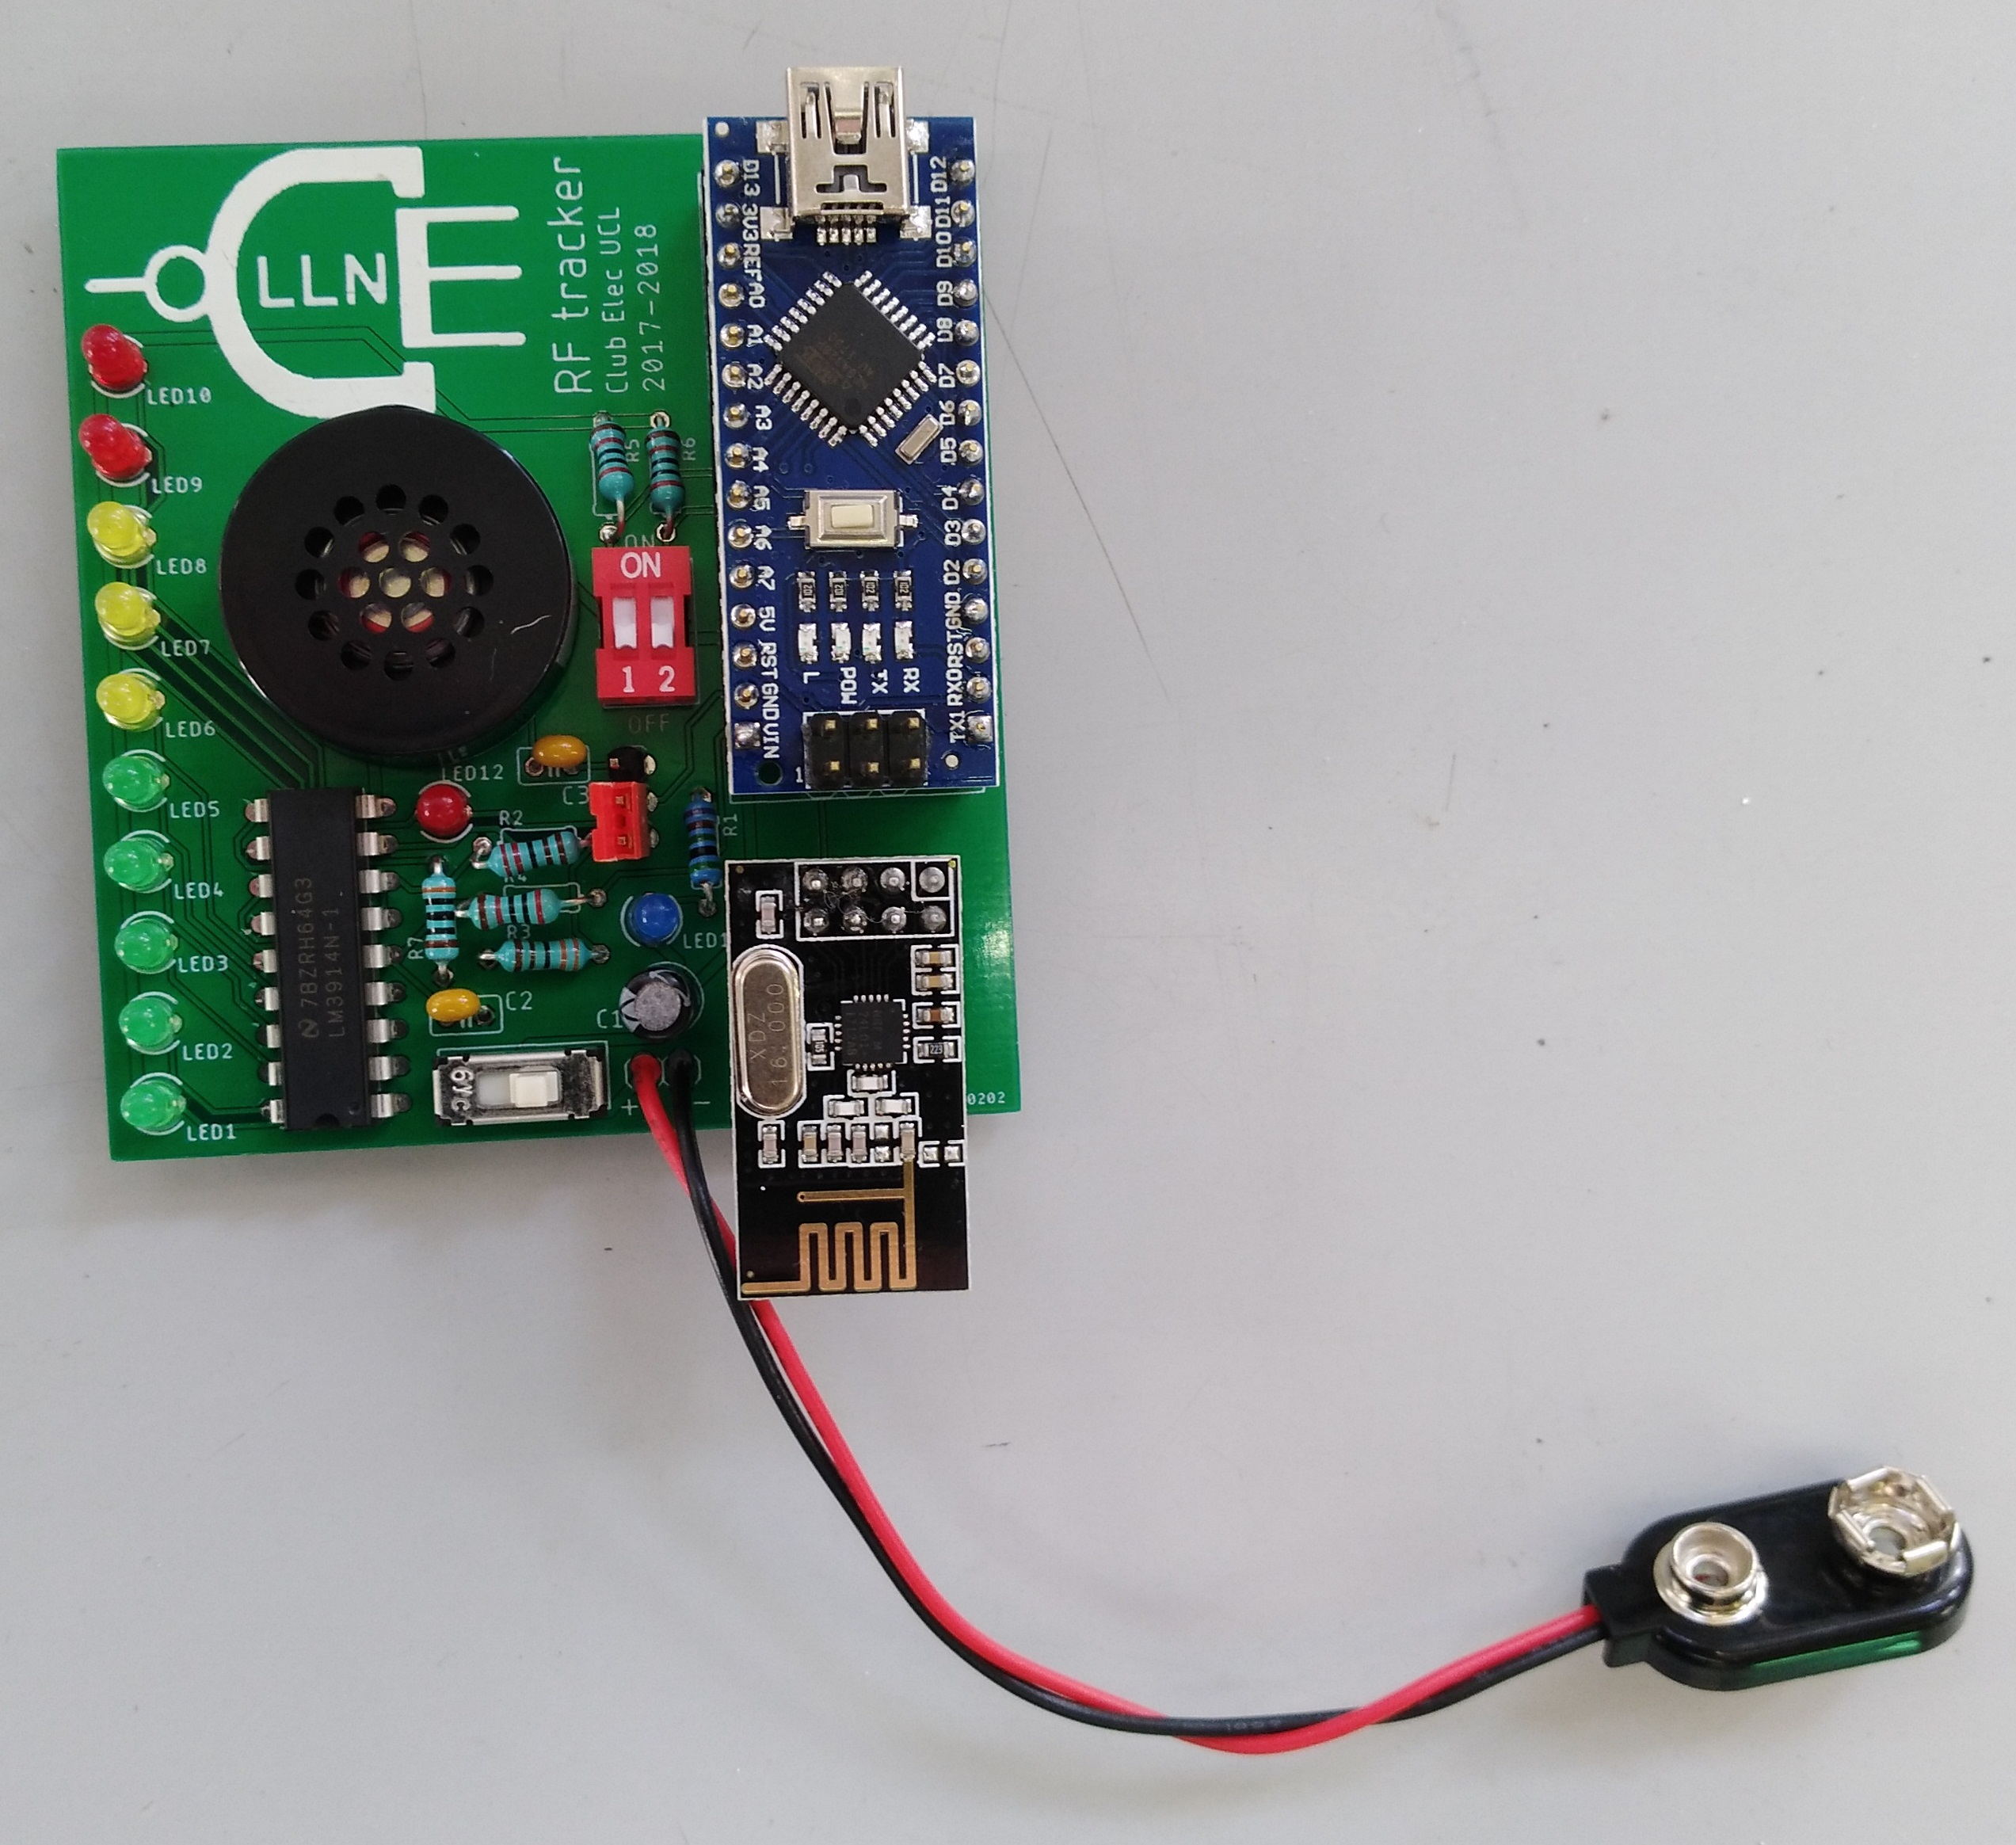
\includegraphics[width=\textwidth]{imgs/RF_TAG.jpg}
	\captionof{figure}{Point d'arrivée : balise RF réceptrice soudée!}
	\label{fig:RF_TAG}
\end{minipage}
\vspace{1cm}

\begin{center}
Bonne lecture, et puisse le sort vous être favorable!
\end{center}

%%% Section 1 : description du système
\section{Description de la balise RF réceptrice}
%%% Principe de fonctionnement du projet
\subsection{Principe de fonctionnement}
Pour déterminer la localisation de la balise émettrice, on se base sur le fait que celle-ci émet des paquets à 4 niveaux de puissance différents. Il semble intuitif que les paquets à plus haut niveau de puissance seront reçus plus loin de la balise que ceux à puissance plus faible. Cela permettra une localisation grossière de l'émetteur. En se rapprochant, davantage de paquets seront reçus par la balise réceptrice, ce qui permettra donc une localisation plus précise de l'émetteur.\\

L'interface fournie par le circuit imprimé permet de visualiser en temps réel le type et la quantité d'information reçue par le récepteur RF. La façon dont les différents composants électroniques seront utilisés dépend de la stratégie choisie par votre groupe, et donc de la programmation du module Arduino Nano.

%%% Schéma-bloc et correspondance sur le PCB
\subsection{Schéma-bloc}
Le schéma-bloc du circuit est présenté à la Fig. \ref{fig:schema-bloc}. Plusieurs niveaux de tensions sont présents pour alimenter les différents composants électroniques constituant le circuit. L'\textbf{alimentation} principale est une pile 9V, qui va alimenter l'Arduino Nano. Celui-ci inclut des régulateurs qui vont produire des tensions de 5V et de 3.3V, utiles aussi pour alimenter les blocs périphériques. Alternativement, l'Arduino peut être alimenté en 5V par une connexion USB.\\

L'\textbf{Arduino Nano} est un composant programmable qui va permettre de contrôler le reste du circuit, selon le code qu'on va venir y placer. Une de ses sorties digitales $DOUT$ est connectée soit au \textbf{buzzer}, soit à une LED, via un jumper. Une de ses sorties analogiques $AOUT$ est connectée au \textbf{driver des LEDs}. Il est également connecté au \textbf{module RF} qui va servir à réceptionner les paquets envoyés par la balise émettrice. Cette connection consiste en une interface de communication de type SPI (Serial Peripheral Interface) comprenant 4 fils, un signal de Chip Enable (CE) et un signal de requête d'interruption (IRQ). Enfin, 2 \textbf{switches} permettent de fixer la valeur de 2 des entrées digitales de l'Arduino, respectivement $DIN1$ et $DIN2$.\\

\begin{figure}[!ht]
	\centering
	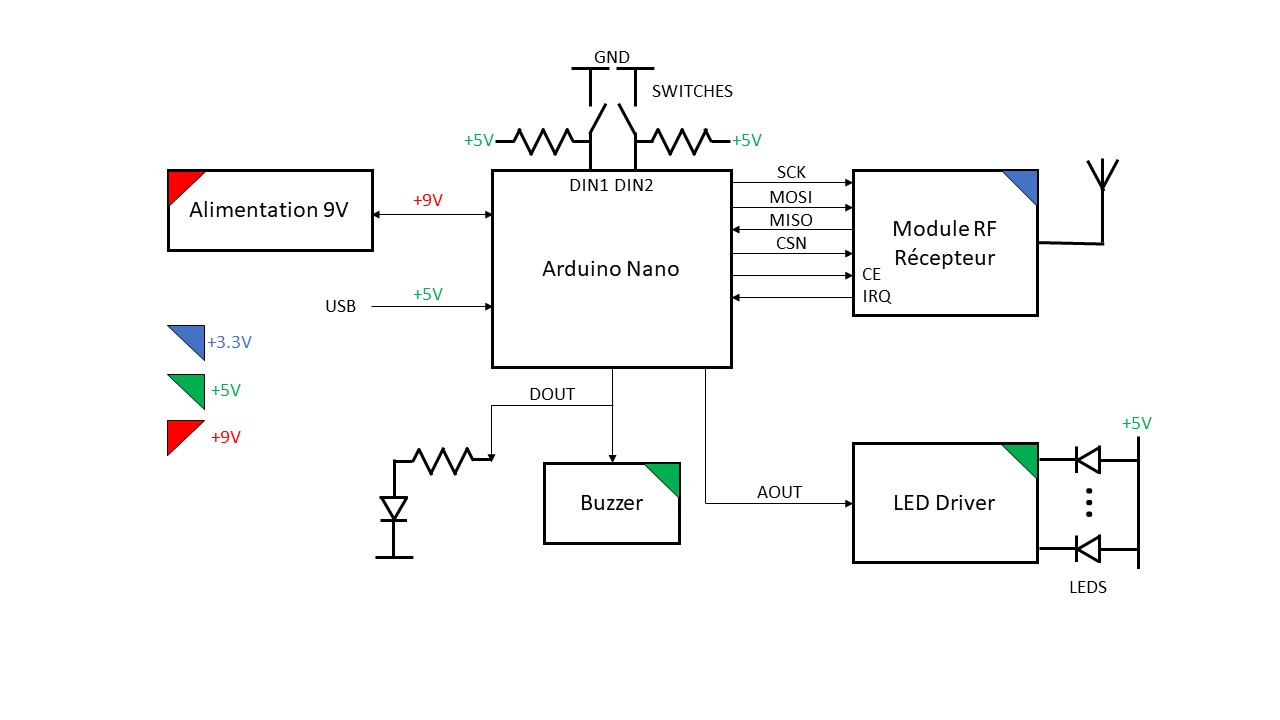
\includegraphics[width=\textwidth]{imgs/schema-bloc.jpg}
	\caption{Schéma-bloc du circuit.}
	\label{fig:schema-bloc}
\end{figure}

\newpage

%%% Description simple des composants principaux
\subsection{Description des composants}
Les composants suivants sont utilisés dans le circuit:\\

\begin{itemize}
\item[$\bullet$] \textbf{Arduino Nano} : Ce composant est essentiel dans le circuit car il permet de contrôler les autres modules. En effet, il peut commander et interagir avec les autres composants électriques (hardware) selon le programme exécuté (software). Il dispose pour cela d'entrées et de sorties analogiques\footnote{En réalité, l'Arduino génère une tension digitale qui est modulée par modulation de largeur d'impulsion (MLI, ou PWM en anglais). Celle-ci est ensuite filtrée par un filtre RC pour donner une tension analogique.} et digitales, ainsi que de protocoles de communication, dans notre cas de type SPI.
\item[$\bullet$] \textbf{Module RF} : Ce module est connecté à l'antenne d'une part et à l'Arduino Nano d'autre part. La communication à l'Arduino consiste en 6 fils. D'abord, les 4 fils du SPI, à savoir l'horloge (SCK), le MOSI (Master Output Slave Input), le MISO (Master Input Slave Output) et le CSN (Chip Select Not). Une entrée CE (Chip Enable) permet l'activation du module, tandis qu'une sortie IRQ (Interrupt Request) permet au module d'interrompre le fonctionnement normal du programme exécuté sur l'Arduino.
\item[$\bullet$] \textbf{Buzzer} : Ce composant est un buzzer de type piézoélectrique. Il est connecté à une des sorties digitales $DOUT$ de l'Arduino. De façon très simplifiée, lorsqu'une tension est appliquée sur ce composant, cela provoque une déformation mécanique qui va produire du son, et donc l'effet "buzzer".
\item[$\bullet$] \textbf{LED driver} : Ce module du circuit va permettre de transformer une tension analogique $AOUT$ produite par l'Arduino en une échelle linéaire représentée par les 10 LEDs qui y sont connectées. 
\item[$\bullet$] \textbf{Switches} : Ces 2 switches permettent de régler la valeur de 2 entrées digitales de l'Arduino, à savoir $DIN1$ et $DIN2$. Lire la valeur de ces entrées peut par exemple servir à choisir entre plusieurs configurations de paramètres du système, à choisir le mode de fonctionnement, etc.\\
\end{itemize}

Ces différents éléments sont identifiés sur la Fig. \ref{fig:RF_TAG_annotated}.\\

\begin{figure}[!ht]
	\centering
	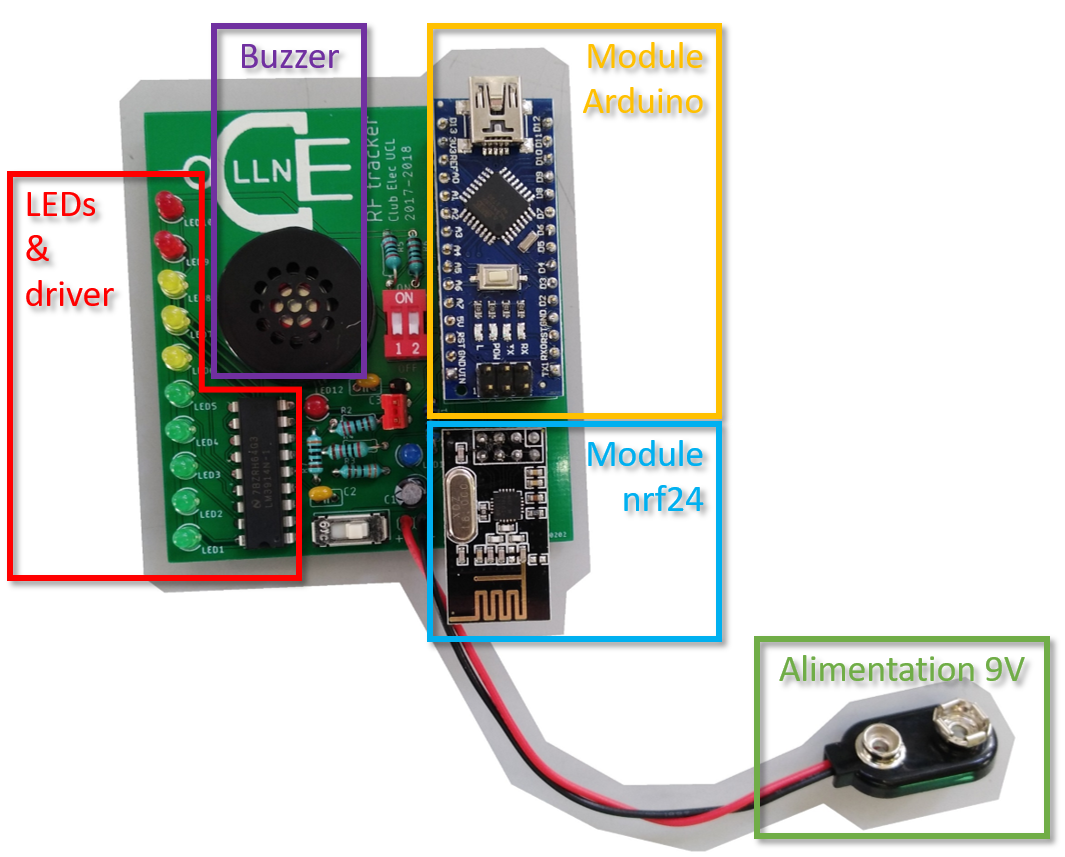
\includegraphics[width=.75\textwidth]{imgs/RF_TAG_annotated.png}
	\caption{Identification des différents blocs sur le circuit imprimé.}
	\label{fig:RF_TAG_annotated}
\end{figure}

%%% Annexes: documents utiles
\newpage
\appendix
\section{Documents utiles}

%%% BoM
\subsection{Liste des composants de la balise}

\begin{table}[!h]
	\centering
	\small
	\begin{adjustbox}{angle=90}
	\begin{tabular}{|c|c|c|c|c|c|c|c|c|}
		\hline
		\textbf{\#} & \textbf{Nom} & \textbf{Nombre} & \textbf{Description} & \textbf{Référence Fabricant} & \textbf{Fabricant} & \textbf{Fournisseur} & \textbf{Prix indicatif [euros]}\\
		\hline
		\hline
		0 & PCB 		& 1 	& Circuit imprimé 			 & - 				& PCB Chart 		& PCB Chart & 4.00\\
		\hline
		\hline
		1  & JP1    	& 1 	& 9V battery holder with cable 	 & 2238        		& Keystone 			& Farnell 	& 0.92\\
		2  & JP2    	& 1 	& 1x3 male pin header, 2.54mm    & 61304011121 		& Wurth Elektronik 	& Farnell 	& 0.11\\  
		3  & pin\_RF 	& 1 	& 2x4 female pin header, 2.54mm  & 2214S-08SG-85 	& Multicomp 		& Farnell 	& 0.41\\ 
		4  & BATT   	& 1 	& 9V 625mAh battery 			 & 6LR61DP12     	& Energizer 		& Farnell 	& 1.77\\ 
		5  & SH	    	& 1 	& Header jumper					 & 2-881545-2    	& AMP  				& Farnell 	& 0.08\\
		6  & S1	    	& 1 	& DIP switches, 2 SPST switches  & MCNDI-02S 		& Multicomp			& Farnell 	& 0.91\\
		7  & S2     	& 1 	& Slide switch, 500mA, SPDT		 & STSSS9121    	& Alps 				& Farnell 	& 0.65\\
		8  & B1     	& 1 	& Buzzer, 100Hz-4kHz, 8ohm       & MCABS-201-RC  	& Multicomp			& Farnell 	& 1.36\\
		9  & IC1    	& 1 	& Led driver, 10 LEDs, 3-15V     & LM3914N       	& Texas Instruments & Farnell 	& 2.33\\
		10 & R1 		& 1 	& Resistor, 700Ohm               & MCMF0W4DF7150A50 & Multicomp 		& Farnell 	& 0.07\\
		11 & R2 		& 1 	& Resistor, 2.2kOhm              & MCMF006FF2201A50 & Multicomp 		& Farnell 	& 0.07\\
		12 & R3 		& 1 	& Resistor, 3.3kOhm              & MCMF006FF3301A50 & Multicomp 		& Farnell 	& 0.07\\
		13 & R4, R5, R6 & 3 	& Resistor, 20kOhm               & MCMF006FF2002A50 & Multicomp 		& Farnell 	& 0.07\\
		14 & R7 		& 1 	& Resistor, 300Ohm               & MCMF006FF3000A50 & Multicomp 		& Farnell 	& 0.07\\
		15 & C1 		& 1 	& Capacitor, 100$\mu$F               & MCUMR6V3107M5X5 	& Multicomp 		& Farnell 	& 0.09\\
		16 & C2, C3 	& 2		& Capacitor, 0.1$\mu$F               & K104K15X7RF53L2	& Vishay 			& Farnell 	& 0.07\\
		\hline
		\hline
		17 & pin\_AN 	& 2 	& 15x1 female pin header, 2.54mm & -  				& COM-FOUR 			& Amazon 	& 0.46\\		
		18 & AN1     	& 1 	& Arduino Nano					 & - 				& Elegoo 			& Amazon 	& 4.00\\		
		19 & RF1      	& 1 	& nRF24L01						 & - 				& Kuman 			& Amazon 	& 2.10\\
		20 & LEDs     	& 12 	& LEDs, various colours 		 & - 				& ILS 				& Amazon 	& 0.16\\
		\hline
	\end{tabular}
	\end{adjustbox}
\end{table}
\newpage
\clearpage

%%% SCHEMATIC
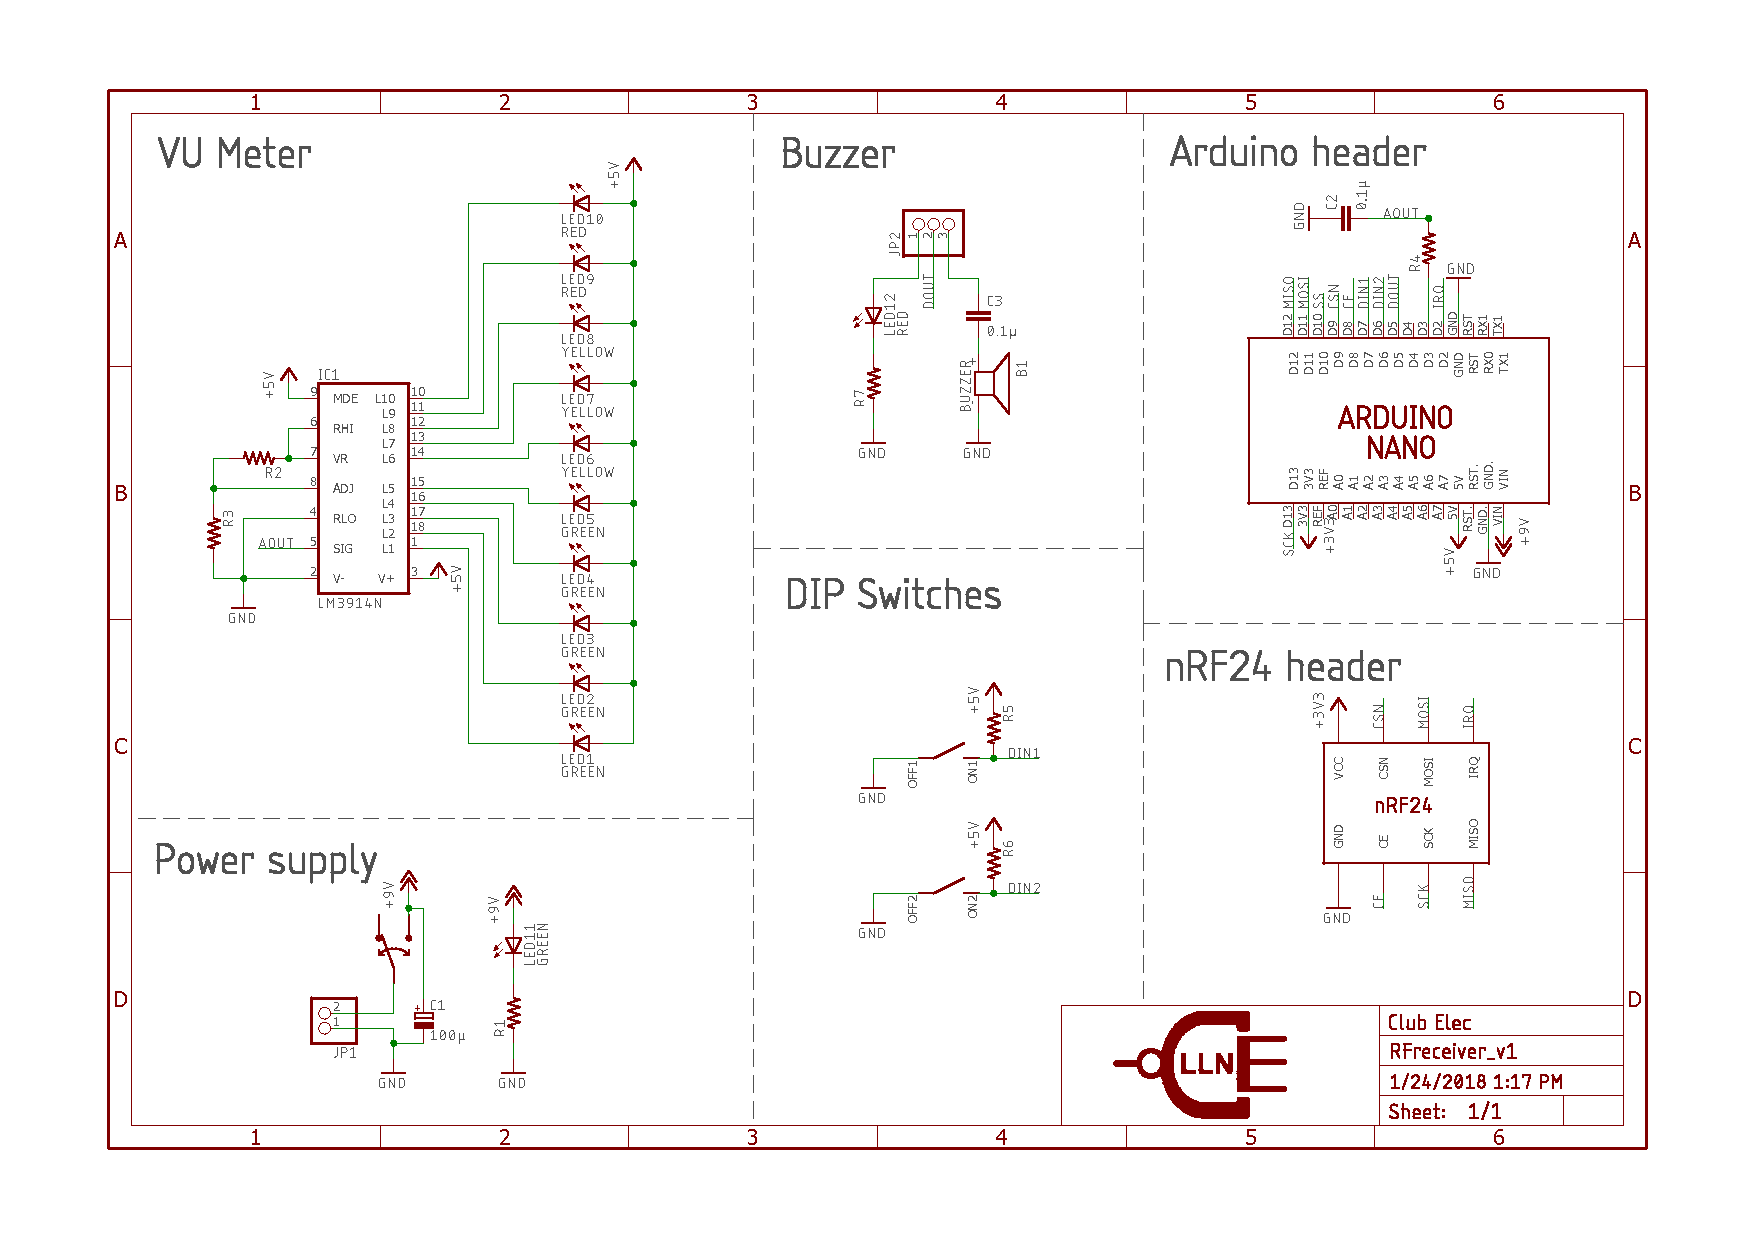
\includepdf[pagecommand=\subsection{Schématique du circuit imprimé}]{RFreceiver_sch.pdf}

%%%  BOARD
\includepdfmerge[nup=1x2,pagecommand=\subsection{Vues physiques du circuit imprimé}]{RFreceiver_brd_top.pdf,RFreceiver_brd_bot.pdf}
\end{document}